\documentclass[a4paper,11pt,oneside]{article}

\usepackage{amsmath,amssymb,epsfig}
\usepackage[T1]{fontenc}
\usepackage{ae,aecompl}
\usepackage{url}
\usepackage{subfigure}
\addtolength{\voffset}{-1cm}
\addtolength{\hoffset}{-1cm}
\setlength{\parindent}{0in}
\addtolength{\textwidth}{1.8cm}
\addtolength{\textheight}{1cm}
\addtolength{\parskip}{.5cm}

% Example definitions.
% --------------------
\def\x{{\mathbf x}}
\def\X{{\mathbf X}}
\def\u{{\mathbf u}}
\def\U{{\mathbf U}}
\def\x{{\mathbf x}}
\def\s{{\mathbf s}}
\def\A{{\mathbf A}}
\def\y{{\mathbf y}}
\def\W{{\mathbf W}}
\def\w{{\mathbf w}}
\def\B{{\mathbf B}}
\def\a{{\mathbf a}}
\def\D{{\mathbf D}}
\def\P{{\mathbf P}}
\def\n{{\mathbf n}}
\def\V{{\mathbf V}}
\def\R{{\mathbf R}}
\def\I{{\mathbf I}}
\def\M{{\mathbf M}}
\def\sech{{\mathrm{sech}}}
\def\L{{\cal L}}
\def\Cum{{\rm{Cum}}}
\def\var{{\rm{var}}}
\def\T{{\mathbf T}}
\def\C{{\mathbf C}}
\def\tf{{\emph{t-f}}}


% Title.
% ------
\title{\large{\textbf{HOMEWORK 3}}}
\author{SGN-1156 Signal Processing Techniques\\
\url{http://www.cs.tut.fi/courses/SGN-1156}\\
Tampere University of Technology\\
Germ\'an G\'omez-Herrero, \url{http://germangh.com}}
\date{Due: November 24, 2009, 10:00 AM}


\begin{document}
\maketitle

\noindent \textbf{Instructions}: Remember to write your name in CAPITAL LETTERS in every page. If you use more than one page you should staple all pages together. You should include in your solutions all relevant intermediate steps. At most you can earn 30 points in this homework. Submit your solutions to mailbox 448 (Tietotalo 4th floor) before the dealine.
\vspace{1cm} 

\noindent \textbf{PROBLEM 1 (10 points):} Consider the system shown in Figure~\ref{fig1}. Assume that the input is bandlimited, $X_a(j\Omega)=0$ for $|\Omega|>2\pi\cdot 500$.

\begin{itemize}
\item[(a)] What constraints must be placed on $M$, $T_1$, and $T_{2}$ in order for $y_a(t)$ to be equal to $x_a(t)$? Sketch the Fourier transforms of $x_a(t)$, $x(n)$, $y(n)$, and $y_a(t)$.
\item[(b)] If $f_1=f_2=10$Khz and $M=2$, find an expression for $y_a(t)$ in terms of $x_a(t)$. What will be the energy of the output signal with respect to the energy of the input signal? \emph{Hint: Assume that the cuttoff frequency of the reconstruction filter is equal to the maximum frequency of the original input signal.}
\end{itemize}

\begin{figure}[h!]
\centering
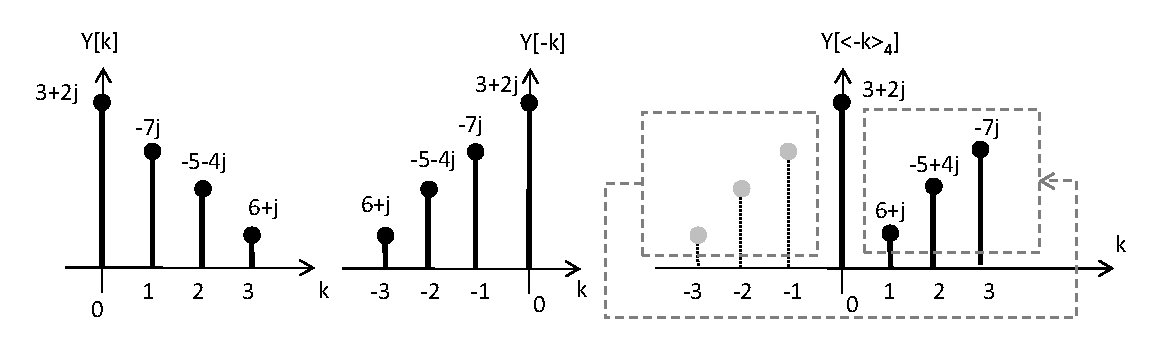
\includegraphics[width=.8\textwidth]{fig1.eps}
\caption{Block diagram of the system of problem 1.}
\label{fig1}
\end{figure}
%
%\begin{figure}[h!]
%\centerline{\subfigure[]{\includegraphics[width=.48\textwidth]{fig1b.eps}
%\label{fig:fig1b}
%}
%\hfil
%\subfigure[]{\includegraphics[width=.4\textwidth]{fig1c.eps}\label{fig:fig1c}
%}
%}
%\caption{Spectrum of the input and frequency response of the digital filter.}
%\label{caca}
%\end{figure}


\vspace{2cm}

\noindent \textbf{PROBLEM 2 (10 points):}  Consider the system on Figure~\ref{fig2} which implements a continuous-time system by sampling, discrete-time system and reconstruction. Assume that the input $x_a(t)$ is bandlimited to $\Omega_{max}=\pi\cdot 5000$. 

\begin{itemize}
\item[(a)] Determine the largest possible value for the sampling period $T$.
\item[(b)] Assume that the sampling period is the one found in part (a). Determine the frequency response $H(e^{j\omega})$ of the discrete-time system, such that the ouput continuous-time signal has the following Fourier transform:
\[
Y_{a}(j\Omega)=\left\{\begin{array}{lll}
\frac{1}{|\Omega|}X_a(j\Omega) & \qquad & 1000\pi \leq |\Omega| \leq 4000\pi\\
0 & \qquad & \textrm{otherwise}
\end{array}\right. 
\]

\item[(c)] If the input signal $x_a(t)$ is a unit variance signal with a completely flat spectrum (i.e. \emph{white noise}), what will be the energy of the output $y_a(t)$?
\end{itemize}


\begin{figure}[h!]
\centering
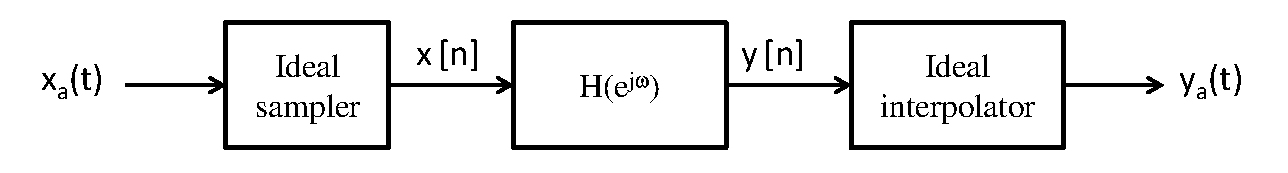
\includegraphics[width=.8\textwidth]{fig2.eps}
\caption{Block diagram of the system of problem 2.}
\label{fig2}
\end{figure}

\vspace{2cm}


\textbf{PROBLEM 3 (10 points):} Diagrammed below is a hybrid digital-analog system:

\begin{figure}[h!]
\centering
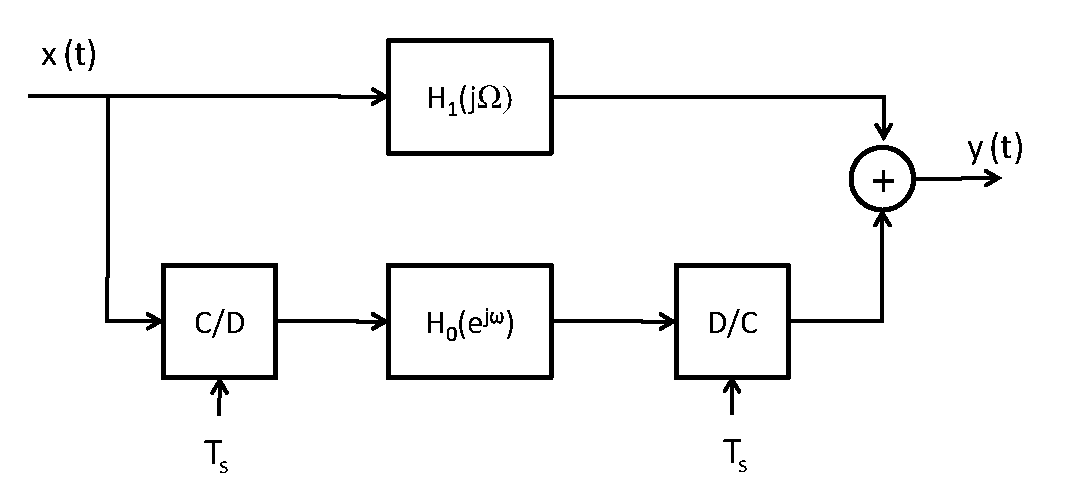
\includegraphics[width=.8\textwidth]{fig4.eps}
\end{figure} 

The discrete-time system is a filter with a frequency response $H_{0}(e^{j\omega})$, which has the shape depicted in Fig.~\ref{fig:filtershape}.

\begin{figure}[h!]
\centering
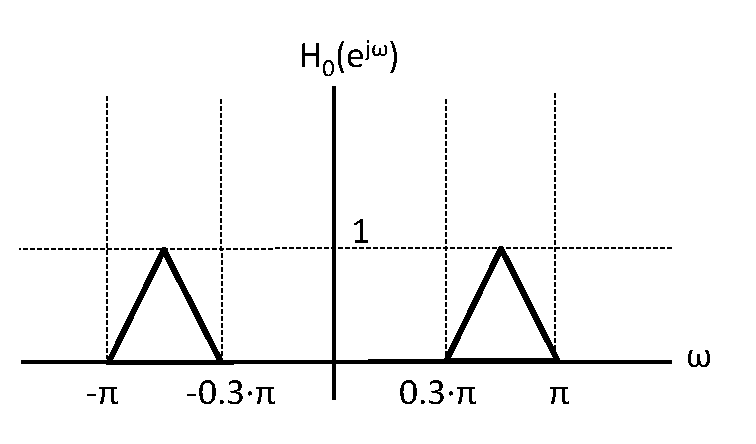
\includegraphics[width=.5\textwidth]{fig5.eps}
\caption{Shape of the filter $H_{0}(e^{j\omega})$ in PROBLEM 3.}
\label{fig:filtershape}
\end{figure} 

The input baseband analog signal is bandlimited to $\Omega_{max}=2\pi\cdot 400$, and the sampling period of the ideal C/D and D/C converters is $T_s=10^{-3}\; s$. Depict the shape that the analog system $H_{1}(j\Omega)$ must have in order to obtain perfect reconstruction, i.e. $y(t)=x(t)$. Specify the numeric value of the relevant frequencies where the shape of $H_{1}(j\Omega)$ changes and the amplitude of $H_{1}(j\Omega)$ at those relevant frequencies. 


\vspace{1cm}

\end{document}